\documentclass[12pt]{article}
\usepackage{CJKutf8}
\usepackage{amsmath, amssymb, amsthm}
\usepackage{graphicx}
\usepackage{dsfont}
\usepackage[natbibapa]{apacite}
\usepackage{geometry}
\geometry{
 a4paper,
 total={210mm,297mm},
 left=30mm,
 right=30mm,
 top=30mm,
 bottom=40mm
}

\title{研究計畫內容:[標題待定]}
\date{}


\begin{document}
\begin{CJK*}{UTF8}{bkai}

\maketitle

\section*{\normalfont(一) 摘要}

\section*{\normalfont(二) 研究動機與研究問題}
民國109年,台灣勞保的給付總額來到將近4.49兆元,其中老年給付就佔了其中的90.4\%,足見
了解老年給付申請誘因之重要。關於勞保年金申請之概況,自民國98年年金化後,年金請領件
數及金額皆呈現穩定成長的趨勢,而一次給付則相對持平如圖一所示。然而,在民國101年及106
年時,一次請領人數明顯上升,可能歸因於政府在此二時間點附近啟動年金改革相關計畫,並伴隨
相關新聞,從而使一次請領人數明顯上升。
\begin{figure}[htbp]
    \centering
    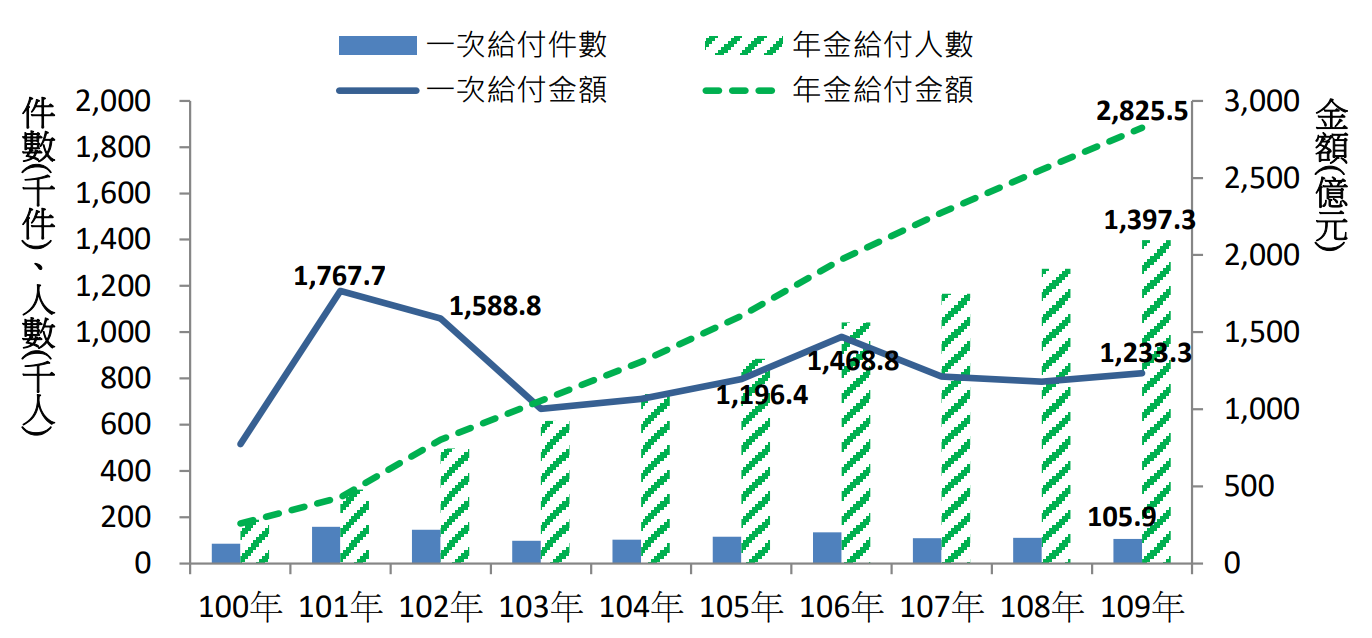
\includegraphics[width=0.8\textwidth]{tw_pension_pay.png}
    \caption{近10年勞保老年給付請領件數及金額(按一次給付及年金給付分)\protect\footnotemark}
\end{figure}
\footnotetext{圖片來源:\cite{old_age_econ5}}

本計畫預計利用財政部財稅資料庫,透過建構異質性個人模型(heterogeneous agent model),
並將個人對於年金改革的信念加入模型之中,以探討年金改革對於勞動供給、儲蓄以及退休年齡之
影響。特別地,本計畫將利用模型進行以下政策實驗:
\begin{enumerate}
    \item 比較民眾對於政府的信任程度不同時,對於年金改革的反應。
    \item 延長退休年齡。
    \item 減少退休金給付。
\end{enumerate}

\section*{\normalfont(三) 文獻回顧與探討}

自\cite{samuelson1958}證明了隨收隨付制(pay-as-you-go, PAYG)可能達成柏拉圖改善以來
\footnote{在一定的條件之下,詳見\cite{aaron1966}},年金制度一向是經濟學家研究的熱門
議題。因文獻眾多且繁雜,本文將以年金制度對於勞動供給、儲蓄以及退休年齡等等的影響為主,
主要聚焦在勞動市場中較為個體層面的影響。

過往美國的研究經常聚焦在退休時間的特殊現象——大多數的退休時間集中在62及65歲。
\cite{burtless1986}與\cite{gustman1986}假設消費者可以無限制地借貸,並假設勞工有異
質的對休閒的偏好,成功地解釋了這個現象。社會安全年金在59到62歲,每推遲一年退休可以增
加終身年金給付725美元;62至65歲之間,每推遲一年退休可以增加807美元的終身年金給付;若
超過65歲,每晚一年退休則僅能增加536美元。這個特別的給付結構使得對於休閒偏好較多的勞工
在62歲時退休,而對於休閒偏好較少的勞工則在65歲時退休。

然而,\cite{stock1990}與\cite{rust1997}指出,前述的特殊現象也可能是因為勞工面臨借貸
限制而產生。

\cite{french2005}將勞動供給、退休以及儲蓄行為內生化,考慮健康、工資的不確定性以及
流動性限制。研究發現年金的請領結構是退休決策的主要因素,若移除對65歲以上的收入檢測制度
\footnote{若收入超過一定水準,政府將會扣留一部份福利,美國在2000年時移除對64歲以上年
齡退休者的收入檢測。}(earnings test),平均退休年齡將延長一年;其餘因素如年金給付額、
健康狀況及借貸限制對高齡退休決策的影響則相對輕微。


\section*{\normalfont(四) 研究方法及步驟}

\subsection*{\normalfont模型}
考慮追求終身效用極大的消費者,其各期效用函數為CRRA,
\begin{equation}
    u(c,n) = \frac{1}{1-\gamma}(c^\eta (l-\theta_n n)^{1-\eta})^{1-\gamma}
\end{equation}
其中$c$為消費、$n$為勞動(假設$n$為離散,$n=1$為有工作;$n=0$則否)、$\theta_n$為工時、
$l-\theta_n n$為休閒、$1-\frac{1}{\eta}$為休閒對消費的替代彈性、$\gamma$為風險厭惡係
數。

工資$w_t$為
\begin{equation}
    \ln w_t = X_t\delta + \epsilon_t
\end{equation}
\begin{equation}
    \epsilon_t \overset{iid}{\sim} N(0,\sigma^2)
\end{equation}
其中$X_t$為個人的特徵如工作年數、性別、教育程度等等。
同時,消費者面對死亡風險$\mu_t$。假設為\cite{thatcher1999}所提出的形式
\begin{equation}
    \mu_t = \frac{\theta_1}{1+ e^{\theta_2 - \theta_3 t}} + \theta_4
\end{equation}
$\theta_1,\theta_3 > 0$且假設存在壽命上限,$\theta_1+\theta_4 > 1$。

消費者面對的預算限制式為
\begin{equation}
    c_t + a_{t+1} = (1+r)a_t + w_t n_t + g(\pi_t,p_t)
\end{equation}
其中$a_t$為$t$期的期初資產、$r$為利率、$\pi_t$為$t$期初勞保累積保額、$p_t$為個人選
擇的退休金計畫($p_t=0$表示尚未領取)、$g(\cdot)$為年金給付之規則。

滿60歲後,消費者可以提領年金,若工作年資滿15年,則可選擇月退休金或一次請領;若工作年資
不滿15年,則只能一次請領。消費者必須在60歲至65歲間選擇退休計畫。

橫截條件(transversality condition)為
\begin{equation}
    \mathbb{E}_t[\frac{a_{T+1}}{(1+r)^T}] = 0
\end{equation}
其中$T$為該消費者死亡年齡。值得一提的是,無龐氏計謀條件(no-Ponzi scheme condition)
\begin{equation}
    \mathbb{E}_t[\frac{a_{T+1}}{(1+r)^T}] \geq 0
\end{equation}
在此模型中提供了自然的流動性限制,借貸限制會隨著年齡增加而緊縮。

另外,我們假設人們具有兩種信念(belief):一種相信年金有較高機率會進行改革\footnote{改革政策
包含延長退休年齡與減少給付等等不同情境,詳見政策實驗一節}($s_i=1$),另一種則較低
($s_i=0$)。每一期消費者認為年金在該期進行改革的機率$q_i$為
\begin{equation}
    q_i = q_0 + q_1 s_i \text{, } s_i \sim Bernoulli(s)
\end{equation}
其中$q_0,q_1 \geq 0$。

消費者有異質的時間偏好率$\beta_i = \alpha_0 + \alpha_1 d_i \text{, } d_i \sim Bernoulli(\beta)$。
最後,假設以上所有除$a_{40}, h_{40}, \pi_{40}$以外的隨機變數互相獨立\footnote{這三個
變數都有initial condition problem,詳見估計一節。}。價值函數(value function)為
\begin{equation}
    \begin{split}
        V_{it}(a_t,h_t,\pi_t,w_t,p_t) = &\max_{c_t,n_t,a_{t+1},\pi^\circ_t,p_t} u(c_t,n_t) \\
        &+ \beta_i (1-\mu_t) \mathbb{E}_t[V_{i,t+1}(a_{t+1},h_{t+1},\pi_{t+1},w_{t+1},p_{t+1})]
    \end{split}
\end{equation}
subject to
\begin{equation}
    c_t + a_{t+1} = (1+r)a_t + w_t n_t + g(\pi_t,p_t)
\end{equation}
\begin{equation}
    \pi_{t+1} = (1+r_p) \pi_t + \pi^f_t - g(\pi_t,p_t)
\end{equation}
\begin{equation}
    \mathbb{E}_t[\frac{a_{T+1}}{(1+r)^T}] = 0
\end{equation}
其中$\pi^f_t$為政府要求雇主每期付出的勞保費用,$r_p$為勞保基金的利率。

\subsection*{\normalfont估計}
為了減輕計算的負擔,我們將採用兩階段的估計方法。第一階段,我們將利用最大
概似估計法(maximum likelihood estimation, MLE)估計死亡率的四個參數
$\Theta = (\theta_1,\theta_2,\theta_3,\theta_4)$。另外,利用\cite{pistaferri2015}
的方法,我們得以將工資的參數$\delta,\sigma$獨立於主要模型的參數進行估計。

第二階段,我們將利用模擬動差估計法(simulated method of moments, SMM)、最大期望算法
(expectation-maximization algorithm, EM algorithm)以及\cite{wooldridge2005}的方法
\footnote{EM algorithm用於處理模型中$s_i,\beta_i$為觀察不到的異質性問題,後者用於處理
initial condition problem。}以估計主要模型的參數
$\Omega = (\gamma,\eta,\alpha_0,\alpha_1,\beta,q_0,q_1,s)$。

\subsection*{\normalfont政策實驗}
\subsubsection*{\normalfont比較民眾對於政府的信任程度不同時,對於年金改革的反應}
在我們的模型之中,異質性$s$可以被視為是整體而言民眾對於政府的信任程度。我們將比較$s=0$
與$s=1$與估計之$s$所模擬出的各項所關心的變數,如勞動供給、儲蓄、退休年齡等等的差異。
\subsubsection*{\normalfont延長退休年齡}
我們將比較延長退休年齡對勞動供給、儲蓄、退休年齡等等的影響。其中,延長退休年齡的方式又
可分為兩種:一種是政府在某期宣布自該期起延長全民退休年齡1年;另一種則是政府在某期宣布自該
期起延長逐步退休年齡,每年以固定的速度延長,如每兩年上調一年等等。
\subsubsection*{\normalfont減少退休金給付}
我們將比較減少退休金給付20\%、50\%與100\%,對勞動供給、儲蓄、退休年齡的影響。

\subsection*{\normalfont研究流程}

\section*{\normalfont(五) 預期結果}
如前所述,本計畫將建構一個異質性個人模型以預測民眾對於年金改革之反應。其次,透過利用模型
進行政策實驗,探討年金改革對於勞動供給、儲蓄以及退休年齡之影響,從而對年金改革之方法提出
建議。
\section*{\normalfont(六) 需要教授指導內容}
\begin{enumerate}
    \item 討論與理解現有文獻,並提出本計畫在文獻中的突破。
    \item 討論模型設定與推導,並完整掌握模型之經濟意義。
    \item 指導計量方法如EM Algorithm、initial conditions problem、
    identification problem等等以及如何加速程式計算。
    \item 指導論文寫作、編排等等。
\end{enumerate}

\bibliographystyle{apacite}
\bibliography{ref_res_app}
\end{CJK*}
\end{document}